\documentclass[DM,authoryear,toc,lsstdraft]{lsstdoc}
\usepackage[nonumberlist,nogroupskip,toc,numberedsection=autolabel]{glossaries}
\makeglossaries
\newacronym[
  description={Continuous Integration. See \S\ref{sec:current:square:ci}.}
]{ci}{CI}{Continuous Integration}

\newacronym[
  description={Key Performance Metric. KPMs are a subset of
  the high-level LSST requirements which were chosen in \citeds{LDM-240}
  to track progress of the DM system towards completion. The current set
  as they pertain to the LST Science Pipelines are described in
  \citeds{LDM-502}. Note that, being derived from high-level requirements,
  KPMs in general describe the performance of the \textit{complete} LSST system,
  and not that of the DM subsystem; it follows that it is impossible to verify
  all KPMs purely based on code and services provided by DM}
]{kpm}{KPM}{Key Performance Metric}

\newglossaryentry{metric}
{
  name={metric},
  description={A measureable quantity which is used to characterize the
  performance of some aspect of the DM system. For example, metrics might
  include photometric repeatability or alert production latency}
}

\newacronym[]{pdac}{PDAC}{Prototype Data Access Center}

\newacronym[]{qa}{QA}{Quality Assurance}

\newacronym[]{qc}{QC}{Quality Control}


\input meta.tex

\title{DM QA Status \& Plans}

\author{%
Simon Krughoff and
John Swinbank
}

\setDocRef{\lsstDocType-\lsstDocNum}
\date{\vcsDate}

\setDocAbstract{%
This document will:

\begin{itemize}

  \item{Describe the current status of ``\gls{qa}'' tools, in the broadest sense,
  currently provided by Data Management;}

  \item{Sketch out a set of common use cases and requirements for future QA
  tool and service development across the subsystem.}

\end{itemize}

It is intended to serve as input to planning for \gls{qa} currently being
undertaken by the DM Leadership Team, the DM System Science Team, and the DM
QA Strategy Working Group (\citeds{LDM-622}).

}

% Change history defined here.
% Order: oldest first.
% Fields: VERSION, DATE, DESCRIPTION, OWNER NAME.
% See LPM-51 for version number policy.
\setDocChangeRecord{%
  \addtohist{1.0 (\vcsRevision)}{\vcsDate}{First release.}{Krughoff \& Swinbank}
}

\begin{document}

\maketitle

\section{Introduction}
\label{sec:intro}

Across the Data Management subsystem, we (ab)use the term ``QA'' to refer to
various aspects of ensuring that things are ``working properly''. This spans a
wide gamut of applications, including, for example:

\begin{itemize}

\item{Does our code correctly compile and pass its unit tests?}
\item{Can we demonstrate that the DM system meets \glspl{kpm} and satisfies
other aspects of our requirements documentation (\citeds{LSE-29, LSE-30,
LSE-61})?}
\item{Do we properly understand the operation of our scientific algorithms,
both individually and operating in concert? Can we identify when the results
they produce are scientifically lacking?}
\item{Do we provide tools to developers, scientists and other members of the
DM team to help them understand and debug the code and systems they are
constructing or using as part of their work?}
\item{How do we track computational performance across the system, from
execution times of scientific algorithms to the scaling properties of database
queries?}
\item{Can we monitor systems within the LSST Data Facility to ensure that they
are operational and performing correctly?}
\item{Can we identify problems which stem from bad data, as distinct from bad
software or services?}

\end{itemize}

To date, the DM team has built a number of tools which address parts of these
problems. However, a coherent, unified vision for how they fit together
remains lacking. This document will\footnote{Ultimately; the current draft
does not yet address all aspects of this scope!} catalogue the tools that are currently
available, will identify use-cases and the requirements arising from them,
will determine to what extent the existing tools satisfy those requirements,
and will suggest directions for future development.

\section{Current Tooling}
\label{sec:current}

We begin by cataloguing the tooling which has been developed to date, or which
will be deployed in the short term\footnote{That is, which we can count on
becoming available shortly, regardless of any future course corrections which
result from this document or other discussion.}. These tools are listed by the
team within DM which originated or leads the development of them.

\subsection{Alert Production (AP)}
\label{sec:current:ap}

\subsubsection{ap\_pipe and ap\_verify}

Development within the Alert Production group has focused on the construction
of an instrumented ``end-to-end'' alert production pipeline.

The pipeline code itself lives in the \code{lsst-dm/ap\_pipe} package in
GitHub. This provides prototype implementations of major alert production
pipeline components (single frame processing, image differencing, source
association), and a control script to string them together\footnote{At time of
writing, this system is being migrated to use the DM-standard
\code{CmdLineTask} framework.}

The \code{lsst-dm/ap\_verify} package is a companion to ap\_pipe. ap\_verify
effectively wraps pipeline functionality in a form that is intended to be
appropriate for regular testing in CI (\S\ref{sec:current:square:ci}). As
such, it provides:

\begin{itemize}

  \item{A standardized way of defining ``dataset'' packages, each of which
  provide a curated test dataset;}
  \item{The facility to ingest data into Butler repositories suitable for
  processing with LSST stack tools;}
  \item{Facilities for instrumenting and calculating \glspl{metric} based upon
  running pipeline code;}
  \item{Submission of calculated \glspl{metric} to SQuaSH using the lsst.verify
  system (\S\S\ref{sec:current:square:squash} \&
  \ref{sec:current:square:verify}).}

\end{itemize}

Based largely upon the experience gained in building ap\_verify, the AP team
has put considerable thought into the appropriate mechanisms for extracting
\glspl{metric} from running pipeline \code{Task}s. This has resulted in
\citeds{DMTN-057}, which describes a number of possibilites for how this might
be standardized. At time of writing, none of these proposals have been
formally adopted by the project.

\subsection{Data Release Production (DRP)}
\label{sec:current:drp}

\subsubsection{\code{afwDisplay}}
\label{sec:current:drp:afwDisplay}

The \code{lsst.afw.display} framework provides a Python API for displaying and
manipulating images and overlaying information source lists based on LSST
stack primitives. The code is backend-agnostic --- that is, the developer
writes to a device-independent common API, and the display can appear on one
of a number of image viewers. Back-end implementations are currently available
for \textit{SAOImage DS9}\footnote{\url{https://github.com/lsst/display_ds9}},
\textit{Matplotlib}\footnote{\url{https://github.com/lsst/display_matplotlib}},
\textit{Firefly}\footnote{\url{https://github.com/lsst/display_firefly}}
(\S\ref{sec:current:suit:firefly}) and
\textit{Ginga}\footnote{\url{https://github.com/lsst/display_ginga}}. Adding
more backends is relatively straightforward. However, the goal of being
backend-agnostic may be in conflict with taking advantage of special
capabilities or functionalities offered by particular tools.

It is worth noting that there is no \code{afwDisplay} equivalent for working
with figures: pipeline developers instead tend to access \textit{Matplotlib}
directly.

The \code{afwDisplay} code does not appear in the work breakdown structure; no
team has formal responsibility for it. However, the DRP team are the primary
maintainers. The teams within science pipelines all make use of \code{afwDisplay}.

\subsubsection{ci\_hsc}
\label{sec:current:drp:cihsc}

The ci\_hsc package provides a curated set of HSC data and a
SCons\footnote{\url{http://www.scons.org/}; note that the choice of SCons here
is ingenious --- it provides many desirable features in a workflow system ---
but also completely non-standard across the rest of the codebase, and can make
this package hard for developers to engage with.}-based system for processing
it through a DRP-like workflow. The resulting data products are automatically
sanity-checked: that is, we establish that the expected outputs have been
produced and contain a plausible number of objects, reasonable selection of
objects used for PSF determination, and so on, but we do not do detailed
analysis of source measurements or astrophyisical plausibility. This means
that ci\_hsc provides an excellent way to catch regressions in pipeline
machinery and integration, but is not sensitive to more subtle algorithmic
issues.

ci\_hsc may be run standalone by individual developers --- it takes around
three hours --- and is periodically run by the CI system
(\S\ref{sec:current:square:ci}).

\subsubsection{Automated static plots with pipe\_analysis}
\label{sec:current:drp:pipeanalysis}

% Text adapted from input from Yusra & the DRP group.
The pipe\_analysis package provides scripts which inspect a repository of
processed data and generate static plots of the distributions of
scientifically relevant quantities. These may be manually inspected to
demonstrate the internal consistency and fidelity of photometric and
astrometric measurements on the visit-stage and coadd-stage catalog outputs.
They also can be used to compare catalog outputs from two different reruns

The plots generated by pipe\_analysis have been refined, and new plots added
to the collection, based on several years of investigating issues encountered
by the DRP group in processing HSC data.

\begin{figure}
\begin{center}
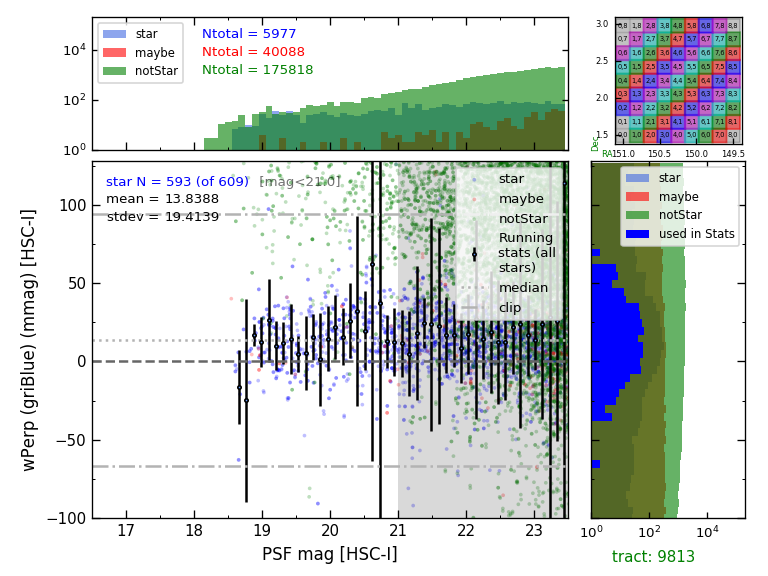
\includegraphics[width=0.48\textwidth]{figures/plot-t9813-color_wPerp-psfMagHist.png}
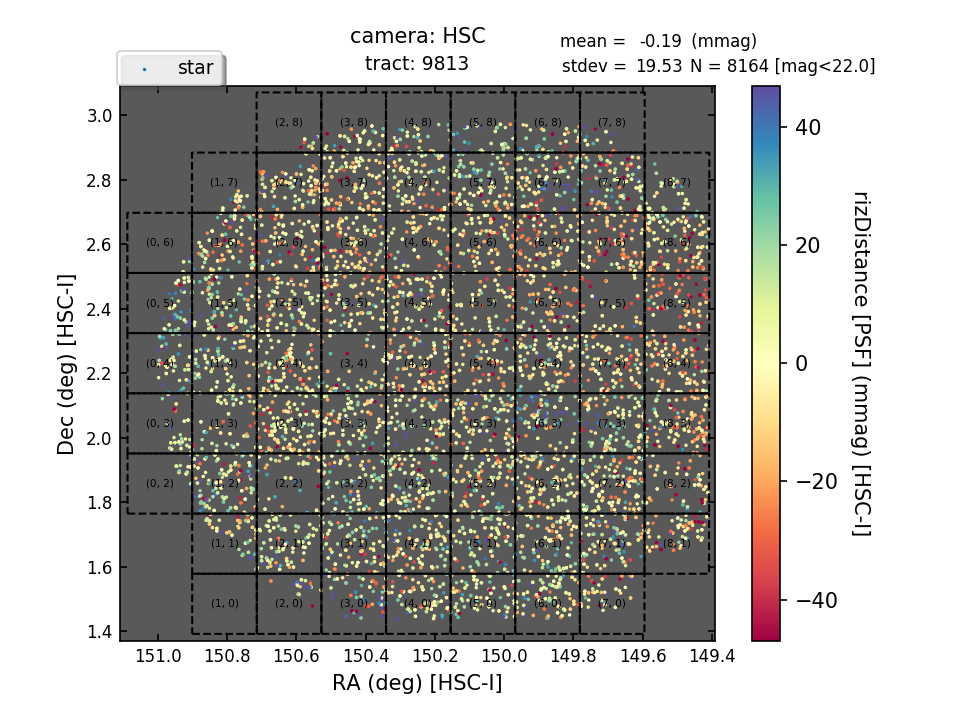
\includegraphics[width=0.48\textwidth]{figures/plot-t9813-rizDistancePSF-sky-stars.png}
\end{center}
\caption{Examples of static plots generated by pipe\_analysis, courtesty of Yusra
AlSayyad.}
\label{fig:pipeanalysis}
\end{figure}

Examples of plots produced by pipe\_analysis are shown in Figure
\ref{fig:pipeanalysis}. Note that this figure shows but two of many plots
generated.

\subsubsection{Dynamic ``drill-down'' plots}
\label{sec:current:drp:drilldown}

% Text adapted from input from Yusra & the DRP group.
Tim Morton (Princeton) is currently building a toolset that offers the ability
to create plots of tracts-worth of catalog data to find patterns and
pathologies. These interactive and linked visualizations, inspired by the
pipe\_analysis plots (\S\ref{sec:current:drp:pipeanalysis}), are created and
explored live in a Jupyter notebook environment.

The current system plotting of multiple quantities of interest, linked to each
other and to sky maps of each quantity; scanning through sky plots of a
quantity from each visit contributing to a coadd; and in-notebook quick-look
of images corresponding to catalog data points.

This toolset is being designed with scalability in mind, and is easily capable
of handling millions of datapoints.

\subsubsection{Large scale scientific analysis of HSC data}
\label{sec:current:drp:hsc}

% Text adapted from input from Yusra & the DRP group.
Approximately annually, a derivate of the LSST codebase is used to process the
full collection of data from the HSC Strategic Survey Program.  This is
coupled with an intensive QA effort (using several of the tools listed above,
in addition to pipeline production scientists in Japan looking at the data) to
verify that new desired features are working as expected and that the
scientific performance of the pipeline has not regressed, before the results
are released to the HSC community. These data releases form the basis of
scientific analyses by the HSC collaboration, which in turn identify issues
that may go unnoticed during pipeline processing.

Processing the entire survey dataset in this way enables the identification of
edge and corner cases that may otherwise go unnoticed.  Unfortunately, the
pipeline outputs are proprietary until they are released to the world a couple
of years later, but members of the DRP team at Princeton can access them and
use the results to trigger development and bug-fixes using public data.

\subsection{Science User Interface \& Tools (SUIT)}
\label{sec:current:suit}

\subsubsection{Firefly}
\label{sec:current:suit:firefly}

\href{https://github.com/Caltech-IPAC/firefly}{Firefly} is the IPAC's ``advanced
astronomy web UI framework''. It provides data browsing, image viewing, and
plotting functionality, and will be the focus of the ``portal aspect'' of the
Science Platform.

Firefly is a client-server application; a Java-based server component is
colocated with the data, and is accessed through a Javascript based UI in the
user's browser. At various times, installations of Firefly have been made
available to DM developers on project-provided compute hardware\footnote{i.e.
\texttt{lsst-dev01.ncsa.illionois.edu}}, but these are not regularly
maintained or accessed by pipelines developers. A firefly server is deployed
with every instance of the JupyterLab environment (\S\ref{sec:current:square:jl}).

Firefly interfaces to the standard image display system used by the LSST
pipelines (\S\ref{sec:current:drp:afwDisplay}) are available.

The functionality available from Firefly may be useful to other DM teams, in
particular providing visualization and plotting services in support of
algorithm development and investigating the properties of data releases.
However, the SUIT team is not scoped to deliver capabilities to the rest of
DM: they are focused on developing Firefly to meet the requirements of the
Science Platform. Other parts of DM may, of course, benefit from the tools
developed for this purpose.

\subsection{Science Data Archive \& Application Services (DAX)}
\label{sec:current:dax}

\subsubsection{Database intgration testing}
\label{sec:current:dax:dbint}

% Text adapted from input from Fritz.
Qserv has a multi-node integration test which spins up several shard servers
and a master via containers, loads a test dataset, and issues a suite of
queries checking against known/expected results. This is run automatically
using the \href{https://travis-ci.org}{Travis CI} service on all changes.

Unfortunately, the nature of this test and the Travis CI service renders it
complicated and brittle; these tests are often broken for reasons unrelated to
a developer's changes. The same test can, however, be run manually by
individual developers before merging.

Larger-scale QServ integration tests are carried out periodically at CC-IN2P3
and the LSST Data Facility. These consist of deploying the containerized Qserv
system across a large cluster and executing queries against large-scale test
datasets. These tests are currently controlled by a collection of scripts, but
work is underway to move to a Kubernetes\footnote{https://kubernetes.io}-based
infrastructure.

\subsubsection{Database performance testing}
\label{sec:current:dax:dbperf}

% Text adapted from input from Fritz.
Performance testing for qserv is performed annually, on synthetic
data sets that are on a glide path to the scale of LSST DR1. The test
procedure is described in \citeds{LDM-552}; examples of the reports produced
include \citeds{DMTR-13} and \citeds{DMTR-16}.

Performance constraints are particualrly an issue for the Level 1 (Prompt)
database prototype. A simulator was developed to test its performance at
various scales. This simualtor is described in \jira{DM-6365}. It is not
regularly run as part of \gls{ci}.

\subsubsection{DAX services}

% Text adapted from input from Fritz.
The current development version of the imgserv service is shipped with an
integrated test suite of several dozen queries, which can be quickly executed
against the service via a built-in CLI, running against either a small test
dataset (included with the code) or the larger data sets currently deployed in
the \gls{pdac}. This same test suite can also be executed directly over
HTTP\footnote{Using a client such as \textit{cURL};
\url{https://curl.haxx.se/}.} to validate the top-end web service layers.

The test suite is not yet integrated with the \gls{ci}
(\S\ref{sec:current:square:ci}) system, but in principle there is no reason
why it could not be.

This testing strategy has been found very successful for imgserv, and
it will be extended to other DAX services as development continues.

\subsubsection{\code{lsstDebug}}
\label{sec:current:dax:debugopt}

% Text adapted from input from Yusra & the DRP group.
The author of an algorithmic task knows which intermediate data products and
diagnostic plots are useful for answering questions about its behavior. The
\code{lsstDebug} framework allows developers to insert code into their
\code{Task}s that displays images (using standard DM primitives) and makes
plots that are only run when the \code{CmdLineTask} is invoked with the
\code{--debug} parameter.

Historically, the \code{lsstDebug} system has been poorly documented and the
subject of some confusion. There are no published guidelines about appropriate
ways to use it or expectations of how developers should instrument their
\code{Task}s.

Note that the \code{lsstDebug} system did not originate with the DAX team
(and, indeed, it's quite likely that no member of DAX has ever used it), but
it falls within their remit as part of the ``task framework''.

\subsection{Data Facility (LDF)}
\label{sec:current:ldf}

\subsubsection{Regular manual reprocessing of HSC data}
\label{sec:current:ldf:hsc}

% Text adapted from input from Yusra & the DRP group.
Every two weeks, members\footnote{Principally Hsin-Fang Chiang} of the LDF
team reprocess some three tracts of HSC data, comprising the ``RC2''
dataset\footnote{The RC2 dataset is fully defined in \jira{DM-11345}.},
through the current weekly release of the DRP pipeline\footnote{Currently,
this means \code{makeSkyMap.py}, \code{singleFrameDriver.py},
\code{mosaic.py}, \code{skyCorrection.py}, \code{coaddDriver.py} and
\code{multiBandDriver.py}.}, including post-processing with the pipe\_analysis
system (\S\ref{sec:current:drp:pipeanalysis}). Any substantive changes in
processing outputs\footnote{For example, changes to CCDs logged as failing
certain pipeline steps, or new errors or exceptions logged during pipeline
operation; we do not consider changes to the contents of the science data
products ``substantive'' for this purpose, as long as those data products are
generated as expected.} are flagged for the attention of the DRP team. The
results of the four most recent processing campaigns are retained for
reference.

In addition, Data Facility staff periodically, on request from the DRP team,
reprocess the whole of the first HSC public data release (``PDR1'') on the
Verification Cluster.

\subsection{Science Quality and Reliability Engineering (SQuaRE)}
\label{sec:current:square}

\subsubsection{Continuous Integration services (Jenkins)}
\label{sec:current:square:ci}

SQuaRE provides and maintains the \href{https://ci.lsst.codes}{CI system}
which regularly builds and tests much of the DM Science Pipelines and Qserv
codebase. The Systems Engineering simulations team also take advantage of the
same system; it is not used by the other teams within DM.

The CI system is widely used for a number of related purposes, including:

\begin{itemize}

  \item{Testing of code by developers before it is merged. Primarily this runs
  all unit tests in all packages, but can also run more comprehensive
  integration tests;}
  \item{Executing \gls{metric} collection systems (e.g. validate\_drp,
  \S\ref{sec:current:square:validate});}
  \item{Building and preparing code for public and internal release. This includes
  packaging both source and binary releases and building Docker images for use in the
  JupyterLab environment \S\ref{sec:current:square:jl}.}

\end{itemize}

\subsubsection{Unit test framework}
\label{sec:current:square:unit}

All code written for DM is expected to be accompanied by appropriate unit
tests\footnote{Refer to the
\href{https://developer.lsst.io/coding/unit_test_policy.html}{Unit Test
Policy} in the \href{https://developer.lsst.io}{Developer Guide}, but note
that our implementation does not follow the terminology it uses}.

The ideal unit test demonstrates that an individual ``unit'' of software (a
class, a function, etc) is operating correctly. In practice, many tests used
by DM go well beyond this, for obvious reasons: it's hard to demonstrate that
the \code{ProcessCcdTask} class is operating correctly without relying on
classes for loading data, performing instrument signature removal, source
detection and measurement, calibration, and so on.  As a natural result of
this, DM's unit tests are often (ab)used to provide mini-integration tests.
While this conflation of integration and unit testing provides convenient test
capabilities which are not easily available elsewhere, it leads to fragility
in the test suite, and makes it impossible, in general, to test modules in a
standalone way: any package needs all of its dependencies available to execute
its test suite.

Although the creation of unit tests is not a responsibility of SQuaRE, the
technology used to implement them, and their regular execution as part of the
CI system, is (although we note that much of the current test harness has been
developed in close cooperation with the Architecture team).

\subsubsection{Stack Demo}
\label{sec:current:square:demo}

The Stack Demo, \code{lsst/lsst\_dm\_stack\_demo}, contains a curated
selection of SDSS data, a script which executes single frame measurement on
that data, and a set of precomputed expected outputs. The results of
measurement are compared with the expected values, and an error is thrown if
any values (including number of detected sources, their positions, and
assorted measurement algorithm results) are different.

Note that the expected values are the results of some previous processing run.
There is no ground truth for this data, and these results have not been
rigorously analysed to demonstrate that they are correct. In short, this
procedure can verify that changes being made do not substantially change the
results of processing, but cannot verify that the results are intrinsically
correct.

The Stack Demo is available for end users to run standalone, but it is also
automatically run as part of most CI (\S\ref{sec:current:square:ci}) jobs.

\subsubsection{lsst.verify}
\label{sec:current:square:verify}

% text adapted from
% https://pipelines.lsst.io/v/DM-11597/modules/lsst.verify/index.html

\href{https://github.com/lsst/verify}{lsst.verify} is a framework for packages
that measure software and data quality \glspl{metric}. A metric can be any
measurable scalar quantity; some examples are in the LSST Science Requirements
Document (\citeds{LPM-17}), though packages can also define ad hoc metrics.
Measurements made through lsst.verify can be uploaded to LSST's SQuaSH
monitoring dashboard (\S\ref{sec:current:square:squash}). The intention behind
the development of \code{lsst.verify} is that it serve as the primary
mechanism for verifying LSST pipelines\footnote{The process of validating the
pipelines in a scientific context are left to the DM validation team.}.

\subsubsection{SQuaSH}
\label{sec:current:square:squash}

\href{https://squash.lsst.codes}{SQuaSH} is a \gls{metric} aggregation and
display service. It provides time-series visualization of selected metrics
derived from \citeds{LDM-502}. Metics may be submitted to SQuaSH using
lsst.verify (\S\ref{sec:current:square:verify}). These metrics are stored and
tracked, making it possible regression alerts to be issued via several
mechanisms including Slack notifications\footnote{Note that this capability
does not seem to be widely advertised or understood.}. All metrics
measurements are accompanied by the associated code changes to aid in
identification of relevant packages in the event of a regression.

To date, the primary use of SQuaSH has been to follow a selection of
\glspl{kpm}.  However, the framework is not restricted to only KPMs: any
metric defined in \code{lsst.verify.metrics} can be uploaded to SQuaSH. SQuaSH
then serves as both a database and search engine for metric measurements as
well as a visualization platform for those measurements.

For a selection of the measuremnts corresponding to select KPMs, specialized
visualiztions have been developed, but it is also possible to query the metric
database\footnote{Using \href{http://graphql.org}{GraphQL}.} for other
measurements to feed to ad hoc visualizations. The intention is that SQuaSH
will be used by developers to track low level metrics on their particular
project as well as higher level Subsystem and Project level metrics.

SQuaSH is described in \citeds{SQR-009}.

\subsubsection{Validation packages}
\label{sec:current:square:validate}


The validate\_drp package will automatically run single-frame processing on a
dataset, calculate a subset of \glspl{metric} derived from the Science
Requirements Document (\citeds{LPM-17}), upload the results to
SQuaSH\footnote{The \code{master} branch of validate\_drp currently uses an
older system for calculating and transmitting \gls{metric} measurements, there
is currently a complete port to the \code{lsst.verify} system on the
\code{verify\_port} branch.}

(\S\ref{sec:current:square:squash}), and evaluate expected analytic models for
photometric and astrometric performance following \cite{2008arXiv0805.2366I}.

It is worth noting that, although these packages are referred to as
``validation'' packages, in fact they form part of the \textit{verification}
process, and will likely be renamed in future.

Currently, validate\_drp supports the following \glspl{metric}\footnote{From
\code{etc/metrics.yaml} of validate\_drp \code{w.2018.07}}:

\begin{itemize}
\item{Relative astrometry
  \begin{itemize}
    \item{AM1, AF1, AD1}
    \item{AM2, AF2, AD2}
    \item{AM3, AF3, AD3}
  \end{itemize}
}
\item{Photometric repeatability
  \begin{itemize}
    \item{PA1, PA2, PF1}
  \end{itemize}
}
\item{Residual PSF ellipticity correlations
  \begin{itemize}
    \item{TE1, TE2}
  \end{itemize}
}
\end{itemize}

The focus, to date, has been on testing data release algorithms, but the
SQuaRE team intends to extend the system to address prompt processing and some
lower level systems (e.g. Jointcal).

In addition, three curated datasets for use with validate\_drp are provided.
These are based on CFHT (validation\_data\_cfht), DECam
(validation\_data\_decam) and HSC (validation\_data\_hsc). These datasets are
reguarly reprocessed by the CI system (\S\ref{sec:current:square:ci}) and the
results uploaded to SQuaSH.

Note that the validation\_data packages contain both ``raw'' data and
processed data which has been ingested to a Butler repository. There is no
regular routine for updating that processed data in light of changes to the
software; developers have occasionally found it unclear or confusing whether
this data is actually supposed to be usable or useful\footnote{In this
context, note \jira{RFC-243} which requests the regular generation of ``a
pipeline output dataset''.}.

\subsubsection{Hosted Jupyter notebooks}
\label{sec:current:square:jl}

The JupyterLab environment is a complete, containerized system for spinning up
Jupyter Notebooks in a hosted environment. The environment comes complete with
pre-compiled recent versions of the stack; currently, these are the three most
recent weekly releases, the two most recent daily releases, and the most
recent major release. The JupyterLab environment provides persistent personal
storage, which may be used to customise the user's personal environment, and
shared storage, which can be used for exchanging data, etc.  It also provides
commonly expected utilites like a shell prompt as well as a text editor.

Currently there are three deployments; all of these target a focused user
community, rather than widespread. These are:

\begin{itemize}

  \item{The DM team developing the JupyterLab system itself;}
  \item{The Systems Engineering team, as they begin commissioning exercises;}
  \item{The Education \& Public Outreach team.}

\end{itemize}

Since these are currently hosted in the on commercial ``cloud'' systems, since
they are relatively small; they are all trivially re-deployable to a project
hosted cluster resource running Kubernetes when such a resource becomes
available.

\section{Requested Functionality}
\label{sec:use}

In this section, we briefly enumerate functionality that has been requested
from across the project under the banner of ``QA''.  We will consider four
broadly separate ``regimes'' in which QA procedures of one sort or another are
relevant:

\begin{description}

\item[Developer support]{Provide developers with the tools they need to work
quicky and effectively when developing scientific algorithms and/or other core
pieces of the system.}

\item[Code quality]{Ensure that our code is buildable, executable, and
maintainable.}

\item[Metric verification]{Demonstrate that we can reliably execute code at
scale and track its performance against predefined targets.}

\item[Science validation]{Check that the results of processing are
scientifically useful, and characterize all the data products produced.}

\end{description}

This brief sketch is not intended to be comprehensive: for a detailed
consideration of DM's sdesires, requirements and future plans for QA, refer to
forthcoming report from the QA Working Group (\citeds{DMTN-085}).

\subsection{Developer Support}

\subsubsection{Test datasets}

When writing code, it is essential that developers have low-friction access to
test datasets from a variety of instruments.

These datasets must be well understood, in terms of their origin and
properties.

It is convenient that such datasets should be available as raw (unprocessed)
data, but also that intermediate and final data products from various stages
of pipeline processing be made available. This facilitiates testing of
algorithms which are only relevant to later parts of the pipeline or analysis
codes (e.g. Jointcal, the Science Platform) without the need for time or
expertise to rerun basic reduction steps.

These processed data products must be kept up-to-date: they should always
correspond to the products that would be produced by the current
state-of-the-art pipeline.

\subsubsection{Visualization, plotting and debugging frameworks}

Although \code{afwDisplay} (\S\ref{sec:current:drp:afwDisplay}) goes some way
towards addressing needs for image display, there is no equivalent for
plotting or displaying catalogue data.

The \code{lsstDebug} system for debugging \code{Task}s is poorly documented
and badly understood, and --- worse --- expectations for how debugging
information should be collected are unclear.

\subsubsection{Support for running and debugging at scale}

Developers request more support with running at scale on e.g. the Verification
Cluster, and, crucially, understanding the results of those runs. Current
debugging techniques consist of little in the way of status information, reams
of unstructured logs, and extensive use of \code{grep}.

\subsubsection{Notifications and dashboards}
\label{sec:requests:notifications}

Many of the systems being described or requested rely on some analysis of the
performance of code being proposed by some particular developer against
standards for code quality, algorithmic correctness, performance, etc.
Wherever possible, the results of these checks should be presented to
developers automatically (e.g. by Slack and/or e-mail notification), and
delivered in a clear and consistent way (rather than requiring developers to
navigate and integrate information from multitudinous chatbots, websites,
and so on).

\subsection{Code quality}

\subsubsection{Unit tests}

Extending unit test coverage and usability protects all developers from code
being broken by changes elsewhere in the stack.

Writing test code that covers complex systems (e.g. \code{Task}s, display
frameworks) can be awkward: better guidance, standards or frameworks for doing
this would reduce the workload on the developer.

The Developer Guide should reflect current best practice and expectations in
respect of testing.

The overloading of unit tests to act as integration tests (as discussed in
\S\ref{sec:current:square:unit}) may contribute to making tests slow and hard
to work with. Stricter guidelines for making unit tests more focused, together
with better integration testing facilities, may help to address this.

\subsubsection{Integration tests}

Integration tests for major DM components should be run regularly. These would
likely include (at a minimum) separate, ``end-to-end'' tests for each of the
alert production and data release production systems, together with other
major components of the system (e.g. alert distribution, databases). Coverage
should be tracked, so that we understand which aspects of the system are being
tested and which are not\footnote{This will include e.g. which \code{Task}s
are not executed by any integration tests because they are disabled by
pipeline configuration.}.

Integration tests are not responsible for scientific validation of data
products. However, they should track all other aspects of execution. This will
likely include:

\begin{itemize}

  \item{Successful execution (the code does not abort or fail);}
  \item{Generation of all expected data products;}
  \item{Significant changes in log messages (e.g. new warnings or errors being
  logged);}
  \item{Changes in data processed, rejected, etc (e.g. some CCDs that
  previously passed now fail);}
  \item{Calculation of \glspl{metric} describing the results.}

\end{itemize}

Note that integration tests may be executed in (at least) two situations:

\begin{itemize}

  \item{Individual developers wish to check their code before a merge;}
  \item{The current \code{master} branch, and any maintained release branches,
  should be regularly exercised to ensure that no regressions have been
  merged.}

\end{itemize}

Note that integration tests which developers are expected to run before
merging to \code{master} must be (relatively) fast to avoid increasing
developer friction.

Checks for regression on \code{master} should be treated with the appropriate
gravity: they should result in notifications
(\S\ref{sec:requests:notifications}) to responsible individuals, and
ultimately be escaled to e.g. the DM Project Manager if they are not
addressed.

\subsubsection{Static analysis, code linters, etc}

A variety of other tools may be applied to identify potential issues or coding
standards violations. While these may often be effective in improving quality,
care must be taken to ensure both that they don't introduce excessive churn
(making e.g. \gls{vcs} history hard to follow) and that the benefits gained
are worth the implementation costs.

\subsection{Metric verification}

\subsubsection{Performance analysis}

Execution time, under controlled conditions\footnote{We might consider whether
AWS instances, or other shared hardware, qualify.}, should be tracked for all
time-sensitive areas of the codebase.

This will obviously include high-level summaries of the time taken to execute
major pipeline components or database queries (which must be tracked in order
to satisfy high-level requirements). However, it must also make it easy to
track the impact of changes to individual algorithms or other components, and
to provide feedback to developers if their changes introduce performance
regressions.

\subsubsection{High-level metric tracking}
\label{sec:requests:kpmtrack}

\Glspl{kpm} derived directly from high-level requirements documents
(\citeds{LPM-17, LSE-29, LSE-30}, etc) are not directly applicable to the DM
codebase, since they characterize the performance of the LSST system
\textit{as a whole}. However, the Subsystem (presumably under the guidance of
the \gls{sst}) should define, and \textit{rigorously} track our performance
against, equivalent quantities that can be well-defined in the context of DM
(for example, measurements made on simulated or precursor datasets).

Actively tracking performance is key. This could take the form of
notifications (\S\ref{sec:requests:notifications}) to key individuals (e.g.
the DM Project Manager, DM Subsystem Scientist, DM Pipelines Scientist, T/CAMs
of relevant groups) on any regression, or a weekly meeting of key personnel to
review collected measurements.

Ultimately, successful verification and delivery of the DM Subsystem is
predicated on hitting predefined targets in all of these \glspl{metric}, and
the DM System Requirements (\citeds{LSE-61}) should be updated to reflect
this.

\subsubsection{Ad-hoc metric calculation and tracking}
\label{sec:requests:adhoctrack}

While some \glspl{metric}, as described in \S\ref{sec:requests:kpmtrack},
should be regularly tracked under controlled conditions on specific datasets,
there is also a need for other metrics to be calculated and --- potentially
--- tracked.

There are a number of considerations here:

\begin{itemize}

  \item{Developers will wish to execute code against arbitrary datasets and
  obtain a high-level summary of its performance. Such metrics might be
  tracked in the short term for developer convenience, but varying compute
  platforms, datasets and algorithmic implementations will render them of
  little value for long-term monitoring.}

  \item{Some ad-hoc metrics should be tracked indefinitely. However, they will
  then require that the platforms and datasets upon which they are being
  tracked are held constant to ensure that the values being recorded are
  comparable with earlier measurements.}

  \item{Interfaces for defining metrics should be made available to
  developers.}

  \item{The types of metric being collected should be considered. From use
  cases collected to date, it's not immediately obvious whether the
  combination of scalar summary values plus the ability to “drill down” to
  processed data products, is adequate, or if more complex datatypes are
  required\footnote{Perhaps equivalent: should the metric-tracking system
  store pipe\_analysis (\S\ref{sec:current:drp:pipeanalysis}-style plots, or
  other intermediate data products, from which summary metric values might be
  derived, in addition to the metric measurements themselves, or should it be
  possible to generate these plots on the fly from the output dataset? If the
  latter, must the output dataset be preserved indefinitely?}.}

\end{itemize}

\subsection{Science validation}

\subsubsection{Drill-down}
\label{sec:requests:drill}

It should be possible to display catalog data or summary metrics of interest
as a function of positio on the sky for (at least) tracts worth of data (and
preferably all sky). When patterns or pathologies are observed, it should be
possible for the user to interactively ``drill down'' to investigate their
source. For example, this includes plotting multiple (user selected)
quantities of interest, enabling brushing \& linking between them, and the
ability to round-trip data to a Jupyter notebook for further analysis. The
tooling should enable the user to investigate questions such as:

\begin{itemize}

\item{Why are the colors in this region of the sky systematically offset from
the stellar locus?}

\item{Why is the difference between CModel Mags and Psf Mags multimodal?}

\item{...}

\end{itemize}

%\section{Requirements}
%\label{sec:req}
%
\printglossary[style=index]

\bibliography{lsst,lsst-dm,refs_ads,refs,books}

\end{document}
